%!TeX encoding = UTF-8
%!TeX program = xelatex
\documentclass[notheorems, aspectratio=54]{beamer}
% aspectratio: 1610, 149, 54, 43(default), 32

\usepackage{latexsym}
\usepackage{amsmath,amssymb}
\usepackage{mathtools}
\usepackage{color,xcolor}
\usepackage{graphicx}
\usepackage{algorithm}
\usepackage{amsthm}
\usepackage{lmodern} % 解决 font warning
% \usepackage[UTF8]{ctex}
\usepackage{animate} % insert gif

\usepackage{lipsum} % To generate test text 
\usepackage{ulem} % 下划线,波浪线

\usepackage{listings} % display code on slides; don't forget [fragile] option after \begin{frame}

% ----------------------------------------------
% tikx
\usepackage{framed}
\usepackage{tikz}
\usepackage{pgf}
\usetikzlibrary{calc,trees,positioning,arrows,chains,shapes.geometric,%
    decorations.pathreplacing,decorations.pathmorphing,shapes,%
    matrix,shapes.symbols}
\pgfmathsetseed{1} % To have predictable results
% Define a background layer, in which the parchment shape is drawn
\pgfdeclarelayer{background}
\pgfsetlayers{background,main}

% define styles for the normal border and the torn border
\tikzset{
  normal border/.style={orange!30!black!10, decorate, 
     decoration={random steps, segment length=2.5cm, amplitude=.7mm}},
  torn border/.style={orange!30!black!5, decorate, 
     decoration={random steps, segment length=.5cm, amplitude=1.7mm}}}

% Macro to draw the shape behind the text, when it fits completly in the
% page
\def\parchmentframe#1{
\tikz{
  \node[inner sep=2em] (A) {#1};  % Draw the text of the node
  \begin{pgfonlayer}{background}  % Draw the shape behind
  \fill[normal border] 
        (A.south east) -- (A.south west) -- 
        (A.north west) -- (A.north east) -- cycle;
  \end{pgfonlayer}}}

% Macro to draw the shape, when the text will continue in next page
\def\parchmentframetop#1{
\tikz{
  \node[inner sep=2em] (A) {#1};    % Draw the text of the node
  \begin{pgfonlayer}{background}    
  \fill[normal border]              % Draw the ``complete shape'' behind
        (A.south east) -- (A.south west) -- 
        (A.north west) -- (A.north east) -- cycle;
  \fill[torn border]                % Add the torn lower border
        ($(A.south east)-(0,.2)$) -- ($(A.south west)-(0,.2)$) -- 
        ($(A.south west)+(0,.2)$) -- ($(A.south east)+(0,.2)$) -- cycle;
  \end{pgfonlayer}}}

% Macro to draw the shape, when the text continues from previous page
\def\parchmentframebottom#1{
\tikz{
  \node[inner sep=2em] (A) {#1};   % Draw the text of the node
  \begin{pgfonlayer}{background}   
  \fill[normal border]             % Draw the ``complete shape'' behind
        (A.south east) -- (A.south west) -- 
        (A.north west) -- (A.north east) -- cycle;
  \fill[torn border]               % Add the torn upper border
        ($(A.north east)-(0,.2)$) -- ($(A.north west)-(0,.2)$) -- 
        ($(A.north west)+(0,.2)$) -- ($(A.north east)+(0,.2)$) -- cycle;
  \end{pgfonlayer}}}

% Macro to draw the shape, when both the text continues from previous page
% and it will continue in next page
\def\parchmentframemiddle#1{
\tikz{
  \node[inner sep=2em] (A) {#1};   % Draw the text of the node
  \begin{pgfonlayer}{background}   
  \fill[normal border]             % Draw the ``complete shape'' behind
        (A.south east) -- (A.south west) -- 
        (A.north west) -- (A.north east) -- cycle;
  \fill[torn border]               % Add the torn lower border
        ($(A.south east)-(0,.2)$) -- ($(A.south west)-(0,.2)$) -- 
        ($(A.south west)+(0,.2)$) -- ($(A.south east)+(0,.2)$) -- cycle;
  \fill[torn border]               % Add the torn upper border
        ($(A.north east)-(0,.2)$) -- ($(A.north west)-(0,.2)$) -- 
        ($(A.north west)+(0,.2)$) -- ($(A.north east)+(0,.2)$) -- cycle;
  \end{pgfonlayer}}}

% Define the environment which puts the frame
% In this case, the environment also accepts an argument with an optional
% title (which defaults to ``Example'', which is typeset in a box overlaid
% on the top border
\newenvironment{parchment}[1][Example]{%
  \def\FrameCommand{\parchmentframe}%
  \def\FirstFrameCommand{\parchmentframetop}%
  \def\LastFrameCommand{\parchmentframebottom}%
  \def\MidFrameCommand{\parchmentframemiddle}%
  \vskip\baselineskip
  \MakeFramed {\FrameRestore}
  \noindent\tikz\node[inner sep=1ex, draw=black!20,fill=white, 
          anchor=west, overlay] at (0em, 2em) {\sffamily#1};\par}%
{\endMakeFramed}

% ----------------------------------------------

\mode<presentation>{
    \usetheme{CambridgeUS}
    % Boadilla CambridgeUS
    % default Antibes Berlin Copenhagen
    % Madrid Montpelier Ilmenau Malmoe
    % Berkeley Singapore Warsaw
    \usecolortheme{beaver}
    % beetle, beaver, orchid, whale, dolphin
    \useoutertheme{infolines}
    % infolines miniframes shadow sidebar smoothbars smoothtree split tree
    \useinnertheme{circles}
    % circles, rectanges, rounded, inmargin
}
% 设置 block 颜色
\setbeamercolor{block title}{bg=red!30,fg=white}

\newcommand{\reditem}[1]{\setbeamercolor{item}{fg=red}\item #1}

% 缩放公式大小
\newcommand*{\Scale}[2][4]{\scalebox{#1}{\ensuremath{#2}}}

% 解决 font warning
\renewcommand\textbullet{\ensuremath{\bullet}}

% ---------------------------------------------------------------------
% flow chart
\tikzset{
    >=stealth',
    punktchain/.style={
        rectangle, 
        rounded corners, 
        % fill=black!10,
        draw=white, very thick,
        text width=6em,
        minimum height=2em, 
        text centered, 
        on chain
    },
    largepunktchain/.style={
        rectangle,
        rounded corners,
        draw=white, very thick,
        text width=10em,
        minimum height=2em,
        on chain
    },
    line/.style={draw, thick, <-},
    element/.style={
        tape,
        top color=white,
        bottom color=blue!50!black!60!,
        minimum width=6em,
        draw=blue!40!black!90, very thick,
        text width=6em, 
        minimum height=2em, 
        text centered, 
        on chain
    },
    every join/.style={->, thick,shorten >=1pt},
    decoration={brace},
    tuborg/.style={decorate},
    tubnode/.style={midway, right=2pt},
    font={\fontsize{10pt}{12}\selectfont},
}
% ---------------------------------------------------------------------

% code setting
\lstset{
    language=C++,
    basicstyle=\ttfamily\footnotesize,
    keywordstyle=\color{red},
    breaklines=true,
    xleftmargin=2em,
    numbers=left,
    numberstyle=\color[RGB]{222,155,81},
    frame=leftline,
    tabsize=4,
    breakatwhitespace=false,
    showspaces=false,               
    showstringspaces=false,
    showtabs=false,
    morekeywords={Str, Num, List},
}

% ---------------------------------------------------------------------

%% preamble
\title[GlobalDataLoader in Multi DeepLearning Task]{GlobalDataLoader in Multi DeepLearning Task}
% \subtitle{The subtitle}
\author{Xie Jian}
\institute[]{I2EC, ICS, NJU}

% -------------------------------------------------------------

\begin{document}

%% title frame
\begin{frame}
    \titlepage
\end{frame}

%% normal frame

% table of content
\begin{frame}
    \frametitle{Table of Contents}
    \tableofcontents
\end{frame}
\AtBeginSection[]
{
    \begin{frame}
        \frametitle{Table of Contents}
        \tableofcontents[currentsection]
    \end{frame}
}
% -----------------------------------------------

\section{Introduction}
\begin{frame}
    \frametitle{DataLoader in Pytorch}
    \begin{center}
        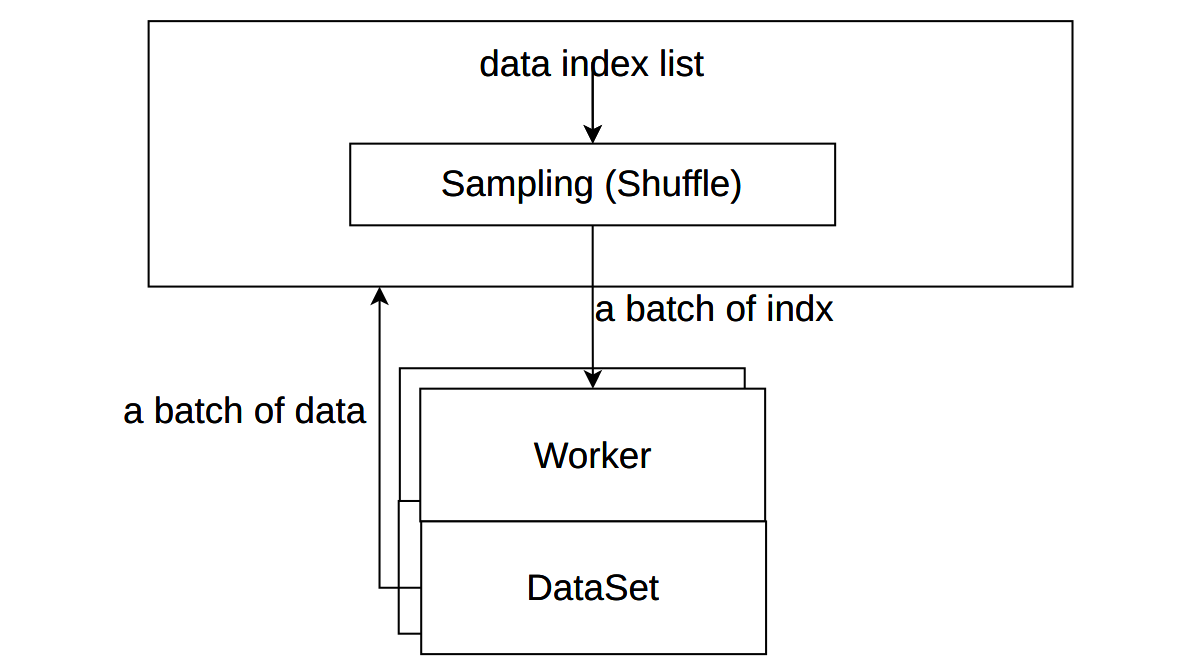
\includegraphics[height=6cm]{global_img_dir/2021-03-02_15-33.png}
    \end{center}
\end{frame}

\begin{frame}
    \frametitle{Problem: Repeated Reading and Processing}
    \begin{block}{Situation}
        To compare the performance of different algorithms, Many DeepLearning tasks are training in the same Dataset.
    \end{block}
    \begin{block}{Problem}
        Every task has its own DataLoader. So the data will be repeatedly read and processed by different tasks.
    \end{block}
    \begin{block}{Result}
        As the number of tasks increases, so does the training time. And what increases is the time to load the data
    \end{block}
\end{frame}

\begin{frame}
    \frametitle{Experiment}
    \begin{figure}[htbp]
    \centering
    \begin{minipage}[t]{0.48\textwidth}
    \centering
    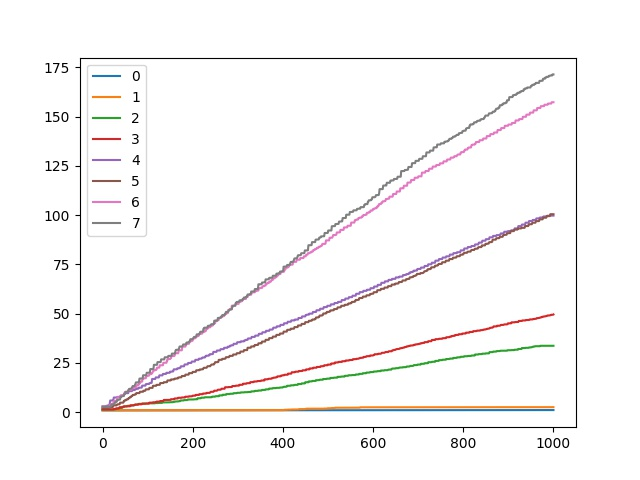
\includegraphics[width=6cm]{global_img_dir/l.jpg}
    \caption{data loading time}
    \end{minipage}
    \begin{minipage}[t]{0.48\textwidth}
    \centering
    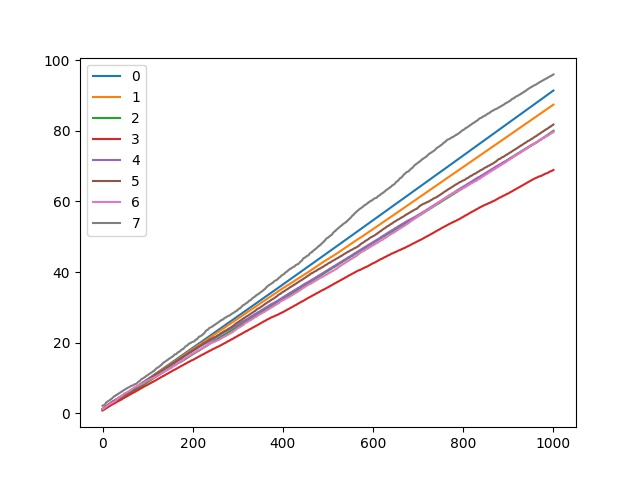
\includegraphics[width=6cm]{global_img_dir/b.jpg}
    \caption{data training time}
    \end{minipage}
    \end{figure}
\end{frame}

\section{Global DataLoader}
\begin{frame}
    \frametitle{Architecture}
    \centering
    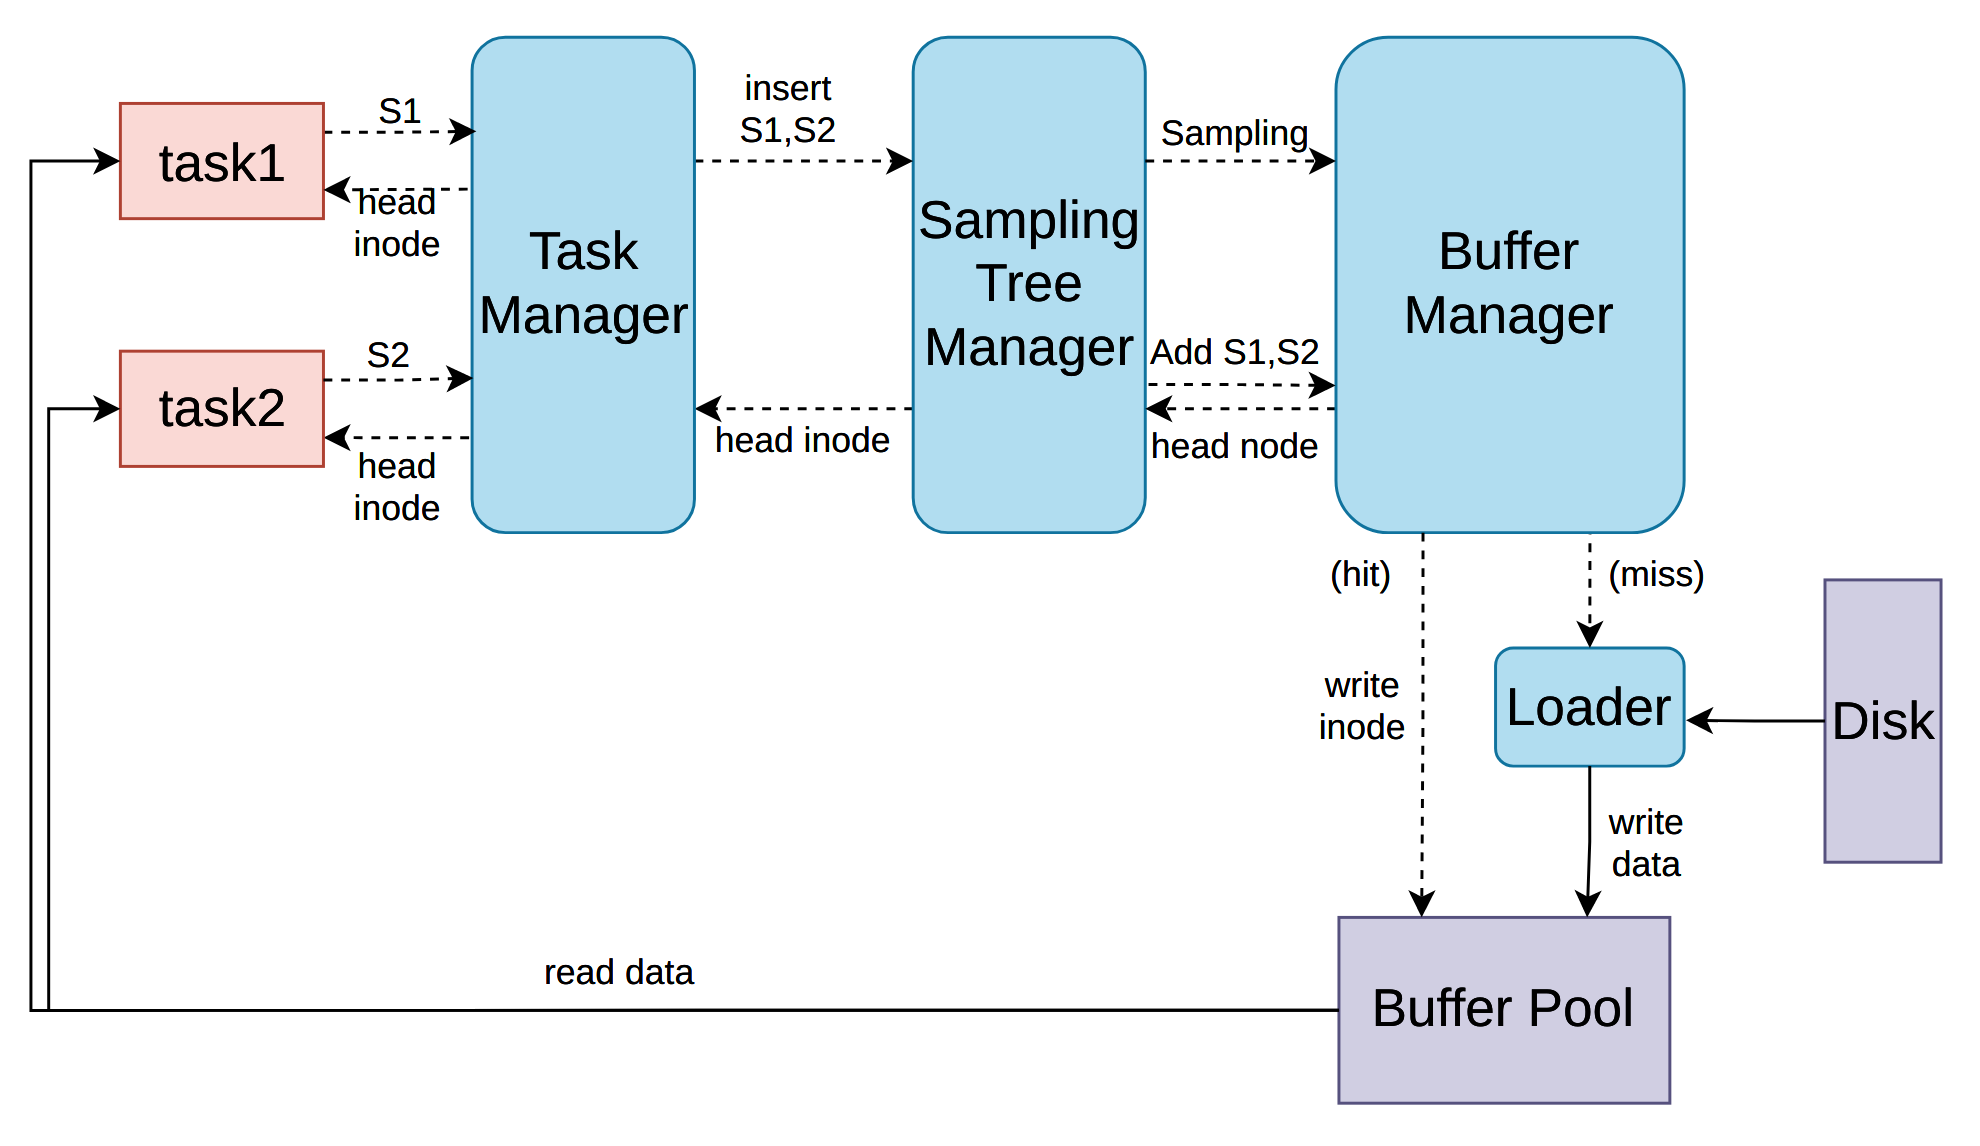
\includegraphics[width=12cm]{global_img_dir/archi.png}
\end{frame}

\begin{frame}
    \frametitle{Sampling: problem description}
    \begin{block}{Defination}
        For a single task, the sampler needs to select an element from the index set $S$.\\
        Similarly, for multiple tasks, the sampler needs to select some elements $\{s_1, s_2, ...\}$ from multiple sets $\{S_1, S_2, ...\}$
    \end{block}
    \begin{block}{Requirments}
        \begin{itemize}
            \item The index in the set $S$ should be randomly sampled. $p(s_i) = \frac{1}{|S_i|}$
            \item Duplicate indexes need to be merged. Maximize the probability $p(s_i = s_j)$
            \item There can be no problem of "starvation"
        \end{itemize}
    \end{block}
\end{frame}

\begin{frame}
    \frametitle{Independently Sampling Algorithm}
    \begin{block}{Assumption}
        There are two sets: $S_1, S_2$, and their length is $n_1, n_2$ \\
        The intersection set of them is $S_i$, whose length is $n_i$ \\
        We divide the set $S_1$ into $S_i$ and $S_{d1} = S_1 - S_i$ \\
        We divide the set $S_2$ into $S_i$ and $S_{d2} = S_2 - S_i$
    \end{block}
    \begin{block}{Example}
        $S_1 = \{1,2,3,4,5\} = \{1,2,3\} \cup \{4,5\}$ \\
        $S_2 = \{1,2,3,6,7\} = \{1,2,3\} \cup \{6,7\}$
    \end{block}
\end{frame}

\begin{frame}
    \frametitle{Independently Sampling Algorithm}
    \begin{block}{Algorithm}
        \begin{itemize}
            \item $S_1$:
            \begin{itemize}
                \item $step_{11}$: randomly select a set from $S_i$ and $S_{d1}$
                \item $step_{12}$: if the set is $S_{d1}$, randomly select a element1 from $S_{d1}$
                \item $step_{13}$: if the set is $S_i$, randomly select a element1 from $S_i$
            \end{itemize}
            \item $S_2$:
            \begin{itemize}
                \item $step_{21}$: randomly select a set from $S_i$ and $S_{d2}$
                \item $step_{22}$: if the set is $S_{d2}$, randomly select a element2 from $S_{d2}$
                \item $step_{23}$: if the set is $S_i$, randomly select a element2 from $S_i$
            \end{itemize}
        \end{itemize}
    \end{block}
    \begin{block}{Probability}
        \begin{equation}
            \begin{aligned}
                p(element1) = \frac{1}{n_1},p(element2) = \frac{1}{n_2}\\
                p(element1 = element2) = \frac{n_i}{n_1*n_2}
            \end{aligned}
        \end{equation}
    \end{block}
\end{frame}

\begin{frame}
    \frametitle{Dependently Sampling Algorithm I}
    \begin{block}{Idea}
        The $step_{13}$ is same as $step_{23}$. We can merge them.
    \end{block}
    \begin{block}{Algorithm}
        \begin{itemize}
            \item $S_1$:
            \begin{itemize}
                \item $step_{11}$: randomly select a set from $S_i$ and $S_{d1}$
                \item $step_{12}$: if the set is $S_{d1}$, randomly select a element1 from $S_{d1}$
                \item $step_{13}$: if the set is $S_i$, go to $step_{33}$
            \end{itemize}
            \item $S_2$:
            \begin{itemize}
                \item $step_{21}$: randomly select a set from $S_i$ and $S_{d2}$
                \item $step_{22}$: if the set is $S_{d2}$, randomly select a element2 from $S_{d2}$
                \item $step_{23}$: if the set is $S_i$, go to $step_{33}$
            \end{itemize}
            \item $step_{33}$: randomly select a element from $S_i$
        \end{itemize}
    \end{block}
\end{frame}

\begin{frame}
    \frametitle{Dependently Sampling Algorithm I}
    \begin{block}{Probability}
        \begin{equation}
            \begin{aligned}
                p(element1) &= \frac{1}{n_1} \\
                p(element2) &= \frac{1}{n_2}\\
                p(element1 = element2) &=  \frac{n_i}{n_1}*\frac{n_i}{n_1} = \frac{n_i^2}{n_1*n_2}
            \end{aligned}
        \end{equation}
    \end{block}
    \begin{block}{Example}
        $S_1 =  \{1,2,3\} \cup \{4,5\}$; $S_2 = \{1,2,3\} \cup \{6,7\}$
        \begin{itemize}
            \item As for $S_1$, select set $\{1,2,3\}$ with probability $0.6$
            \item As for $S_2$, select set $\{1,2,3\}$ with probability $0.6$
            \item Finally, randomly sampling element in $\{1,2,3\}$
            \item $p(element1 = element2) = 0.6*0.6 = 0.36$
        \end{itemize}
    \end{block}
\end{frame}

\begin{frame}
    \frametitle{Dependently Sampling Algorithm I}
    \begin{block}{Idea}
        The $step_{11}$ and $step_{21}$ are similar. We can merge them.
    \end{block}
    \begin{block}{Algorithm}
        \begin{itemize}
            \item $step_{1}$: randomly select a set from $S_i$ and $S_{d1}$
            \item $S_1$:
            \begin{itemize}
                \item $step_{12}$: if the set is $S_{d1}$, randomly select a element1 from $S_{d1}$
                \item $step_{13}$: if the set is $S_i$, go to $step_{33}$
            \end{itemize}
            \item $S_2$:
            \begin{itemize}
                \item $step_{22}$: if the set is not $S_{d1}$, randomly select a element2 from $S_{d2}$
                \item $step_{23}$: if the set is $S_i$, go to $step_{33}$
            \end{itemize}
            \item $step_{33}$: randomly select a element from $S_i$
        \end{itemize}
    \end{block}
\end{frame}

\begin{frame}
    \frametitle{Problem}
    \begin{block}{Probability}
        As for $S_1$:
        \begin{equation}
            \begin{aligned}
                p_1(S_i) &= \frac{n_i}{n_1} \\
                p_1(S_{d1}) &= 1-\frac{n_i}{n_1}
            \end{aligned}
        \end{equation}
        As for $S_2$:
        \begin{equation}
            \begin{aligned}
                p_2(S_i) &= \frac{n_i}{n_2} \\
                p_2(S_{d2}) &= 1-\frac{n_i}{n_2}
            \end{aligned}
        \end{equation}
    \end{block}
    \begin{block}{Problem}
        if $n_1 \neq n_2$, \\
        then $p_1(S_i) \neq p_2(S_i)$ and $p_1(S_{d1}) \neq p_2(S_{d2})$
    \end{block}
\end{frame}

\begin{frame}
    \frametitle{Case1: n1 < n2}
    \begin{block}{Problem}
        \begin{equation}
            \begin{aligned}
                (p_1(S_i) = \frac{n_i}{n_1}) > (p_2(S_i) = \frac{n_i}{n_2}) \\
            \end{aligned}
        \end{equation}
    \end{block}
    \begin{block}{Approach}
        So in $step_1$, when select $S_i$, it should be changed $S_{d2}$ in probability of $p$. \\
        The equation is 
        \begin{equation}
            \begin{aligned}
                p_2(S_i) &= p_1(S_i)*(1-p) = \frac{n_i}{n_2} \\
                p_2(S_{d2}) &= p_2(S_{d1})+p_1(S_i)*{p} = 1-\frac{n_i}{n_2}
            \end{aligned}
        \end{equation}
        then
        $$p = 1-\frac{n_1}{n_2}$$
    \end{block}
\end{frame}

\begin{frame}
    \frametitle{Dependently Sampling Algorithm II}
    \begin{block}{Algorithm}
        \begin{itemize}
            \item $step_{1}$: randomly select a set $S$ from $S_i$ and $S_{d1}$
            \item $S_1$:
            \begin{itemize}
                \item $step_{12}$: if the $S$ is $S_{d1}$, randomly select a element1 from $S_{d1}$
                \item $step_{13}$: if the $S$ is $S_i$, go to $step_{3}$
            \end{itemize}
            \item $S_2$:
            \begin{itemize}
                \item $step_{22}$: if the $S$ is $S_{d2}$, randomly select a element2 from $S_{d2}$
                \item $step_{23}$: if the $S$ is $S_i$
                \begin{itemize}
                    \item randomly let $S = S_{d1}$ in probability of $1-\frac{n_1}{n_2}$
                    \item if $S$ is $S_{d2}$, randomly select a element2 from $S_{d2}$
                    \item if $S$ is $S_i$, go to $step_{3}$
                \end{itemize}
            \end{itemize}
            \item $step_{3}$: randomly select a element from $S_i$
        \end{itemize}
    \end{block}
\end{frame}

\begin{frame}
    \frametitle{Dependently Sampling Algorithm II}
    \begin{block}{Probability}
        % If in $step_1$, the selected set $S = S_i$, and $p_1(S_i) = \frac{n_i}{n_1}$
        % $$
        %     p(element2) = p_1(S_i)*(\frac{n_1}{n_2})*\frac{1}{n_i} = \frac{1}{n_2}
        % $$
        % If in $step_1$, the selected set $S = S_{d1}$, and $p_1(S_{d1}) = 1-\frac{n_i}{n_1}$
        % $$
        %     p(element2) = (p_1(S_{d1})+(1-\frac{n_1}{n_2})*p_1(S_i))*\frac{1}{n_2-n_i} = \frac{1}{n_2}
        % $$
        % and
        $$
            p(element1 = element2) = p_1(S_i)*(\frac{n_1}{n_2}) = \frac{n_i}{n_2}
        $$
    \end{block}
    \begin{block}{Example}
        $S_1 =  \{1,2,3\} \cup \{4\}$; $S_2 = \{1,2,3\} \cup \{6,7\}$
        \begin{itemize}
            \item In $step_1$, select set $\{1,2,3\}$ with probability $\frac{3}{5} = 0.75$
            \item Then as for $S_2$, select set $\{1,2,3\}$ with probability $\frac{4}{5}=0.8$
            \item Finally, randomly sampling element in $\{1,2,3\}$
            \item $p(element1 = element2) = 0.75*0.8=0.6$
        \end{itemize}
    \end{block}
\end{frame}

\begin{frame}
    \frametitle{Case1: n1 > n2}
    \begin{block}{Problem}
        \begin{equation}
            \begin{aligned}
                (p_1(S_{d1}) = 1-\frac{n_i}{n_1}) > (p_2(S_{d_2}) = 1-\frac{n_i}{n_2}) \\
            \end{aligned}
        \end{equation}
    \end{block}
    \begin{block}{Approach}
        So in $step_1$, when select $S_{d1}$, it should be changed $S_{i}$ in probability of $p$. \\
        The equation is 
        \begin{equation}
            \begin{aligned}
                p_2(S_i) &= p_1(S_i)+p_2(S_{d1})*p = \frac{n_i}{n_2} \\
                p_2(S_{d2}) &= p_2(S_{d1})*(1-p) = 1-\frac{n_i}{n_2}
            \end{aligned}
        \end{equation}
        then
        $$p = 1-\frac{n1*(n2-n_c)}{n2*(n1-n_c)}$$
    \end{block}
\end{frame}

\begin{frame}
    \frametitle{Dependently Sampling Algorithm II}
    \begin{block}{Algorithm}
        \begin{itemize}
            \item $step_{1}$: randomly select a set $S$ from $S_i$ and $S_{d1}$
            \item $S_1$:
            \begin{itemize}
                \item $step_{12}$: if the $S$ is $S_{d1}$, randomly select a element1 from $S_{d1}$
                \item $step_{13}$: if the $S$ is $S_i$, go to $step_{3}$
            \end{itemize}
            \item $S_2$:
            \begin{itemize}
                \item $step_{22}$: if the $S$ is $S_{d2}$, randomly select a element2 from $S_{d2}$
                \begin{itemize}
                    \item randomly let $S = S_{i}$ in probability of $1-\frac{n1*(n2-n_c)}{n2*(n1-n_c)}$
                    \item if $S$ is $S_{d2}$, randomly select a element2 from $S_{d2}$
                    \item if $S$ is $S_i$, randomly select a element2 from $S_{i}$
                \end{itemize}
                \item $step_{23}$: if the $S$ is $S_i$, go to $step_3$
            \end{itemize}
            \item $step_{3}$: randomly select a element from $S_i$
        \end{itemize}
    \end{block}
\end{frame}

\begin{frame}
    \frametitle{Dependently Sampling Algorithm II}
    \begin{block}{Probability}
        % If in $step_1$, the selected set $S = S_i$
        % $$
        %     p(element2) = (p_1(S_i)+p_2(S_{d1})*p)*\frac{1}{n_i} = \frac{1}{n_2}
        % $$
        % If in $step_1$, the selected set $S = S_{d1}$, and $p_1(S_{d1}) = 1-\frac{n_i}{n_1}$
        % $$
        %     p(element2) = ( p_2(S_{d1})*(1-p))*\frac{1}{n_2-n_i} = \frac{1}{n_2}
        % $$
        % and
        $$
            p(element1 = element2) = p_1(S_i)) = \frac{n_i}{n_1}
        $$
    \end{block}
    \begin{block}{Example}
        $S_1 =  \{1,2,3\} \cup \{4,5\}$; $S_2 = \{1,2,3\} \cup \{6\}$
        \begin{itemize}
            \item In $step_1$, select set $\{1,2,3\}$ with probability $\frac{3}{4} = 0.6$
            \item Then $S_2$ must select $\{1,2,3\}$
            \item Finally, randomly sampling element in $\{1,2,3\}$
            \item $p(element1 = element2) = 0.6$
        \end{itemize}
    \end{block}
\end{frame}

% \begin{frame}
%     \frametitle{Dependently Sampling Algorithm II}
%     \begin{block} {step1}
%         $step_{1}$: randomly select a set $S$ from $S_i$ and $S_{d1}$
%     \end{block}
%     \begin{block}{$step_2: S_1$}
%         \begin{itemize}
%             \item $step_{12}$: if the $S$ is $S_{d1}$, randomly select a element1 from $S_{d1}$
%             \item $step_{13}$: if the $S$ is $S_i$, go to $step_{3}$
        
%             \item $step_{3}$: randomly select a element from $S_i$
%         \end{itemize}
%     \end{block}
%     \begin{block}{$step_2:S_2$}
%         \begin{itemize}
%             \item $step_{22}$:
%             \begin{itemize}
%                 \item if $n_1 > n_2$:
%                 \begin{itemize}
%                     \item 
%                 \end{itemize}
%                 % \begin{itemize}
%                     % \item 
%                 % \item randomly let $S = S_{d1}$ in probability of $1-\frac{n_1}{n_2}$
%                 % \item if $S$ is $S_{d2}$, randomly select a element2 from $S_{d2}$
%                 % \item if $S$ is $S_i$, go to $step_{3}$
%                 % \end{itemize}
%             \end{itemize}
%             \item $step_{23}$: if the $S$ is $S_i$
%             \begin{itemize}
%                 \item randomly let $S = S_{d1}$ in probability of $1-\frac{n_1}{n_2}$
%                 \item if $S$ is $S_{d2}$, randomly select a element2 from $S_{d2}$
%                 \item if $S$ is $S_i$, go to $step_{3}$
%             \end{itemize}
%         \end{itemize}
%     \end{block}
% \end{frame}

\begin{frame}
    \frametitle{Why not shuffle $S_1 \cup S_2$}
    \begin{block} {Probability}
        $p(element1=element2) = \frac{|S_1\cap S_2|}{|S_1 \cup S_2|} < \frac{|S_1\cap S_2|}{max(|S_1|,|S_2|)}$
    \end{block}
    \begin{block} {randomly select in $S_1\cup S_2$: "starvation"}
        if $|S_1| = 99, |S_2| = 1$,
        then $p(element \in S_1) = 0.99, p(element \in S_2) = 0.01$ \\
        So task2 may be starving
    \end{block}
    \begin{block} {shuffle $S_1\cup S_2$: offset}
        $S_1 = \{3,4\}, S_2 = \{1,3,4\}$\\
        \{\space \space \space \space 3,4\}\\
        \{1,2,3,4\} \\
        \{1,\space \space 3,4\}\\
    \end{block}
\end{frame}

\begin{frame}
    \frametitle{Sampling Tree}
    \begin{block} {Attributes}
        \begin{itemize}
            \item There are two sets $S_1, S_2$ and $n_1 > n_2$
            \item $S_a = S_a\cap S_b$, whose length is $n_a$
            \item $S_b = S_1- S_a$, whose length is $n_b$
            \item $S_c = S_2- S_a$, whose length is $n_c$
        \end{itemize}
    \end{block}
    \centering
    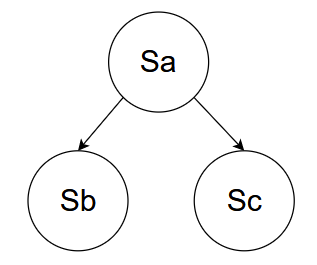
\includegraphics[width=5cm]{global_img_dir/SamplingTree1.png}
\end{frame}

\begin{frame}
    \frametitle{case1 and case2}
    \begin{block}{Algorithm}
        \begin{itemize}
            \item case1: $p_1 \leq n_a/n_1$  and  $p_2 \leq n1/n_2$
            \begin{itemize}
                \item $S_a = S_a - \{a\}$
            \end{itemize}
            \item case2: $p_1 > n_a/n_1$:
            \begin{itemize}
                \item $S_b = S_a - \{b\}$
                \item $S_c = S_c - \{c\}$
            \end{itemize}
        \end{itemize} 
    \end{block}
    \begin{figure}[htbp]
        \centering
        \begin{minipage}[t]{0.48\textwidth}
        \centering
        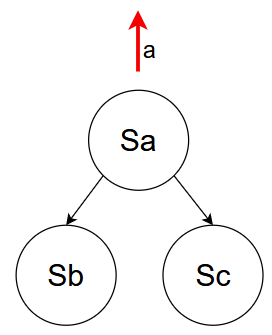
\includegraphics[width=3cm]{global_img_dir/Sampling1.png}
        \caption{case1}
        \end{minipage}
        \begin{minipage}[t]{0.48\textwidth}
        \centering
        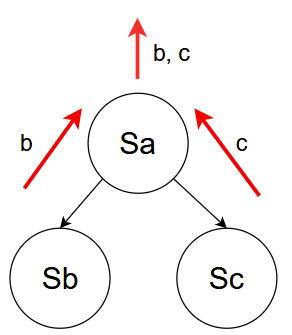
\includegraphics[width=3cm]{global_img_dir/Sampling2.png}
        \caption{case2}
        \end{minipage}
    \end{figure}
\end{frame}

\begin{frame}
    \frametitle{case3 and case4}
    \begin{block}{Algorithm}
        \begin{itemize}
            \item case3: $p_1 \leq n_a/n_1$  and  $p_2 > n1/n_2$
            \begin{itemize}
                \item $S_b = S_b - \{b\}$
                \item $S_c = S_c \cup \{a\} - \{c\}$
            \end{itemize}
        \end{itemize} 
    \end{block}
    \begin{figure}[htbp]
        \centering
        \begin{minipage}[t]{0.48\textwidth}
        \centering
        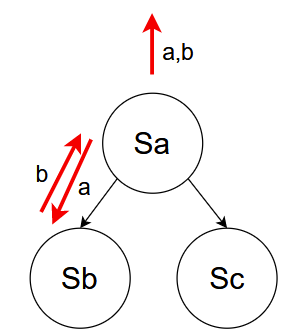
\includegraphics[width=3cm]{global_img_dir/Sampling3.png}
        \caption{impossible}
        \end{minipage}
        \begin{minipage}[t]{0.48\textwidth}
        \centering
        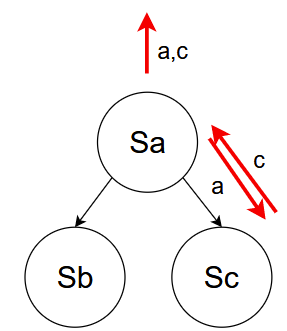
\includegraphics[width=3cm]{global_img_dir/Sampling4.png}
        \caption{case3}
        \end{minipage}
    \end{figure}
\end{frame}

\begin{frame}
    \frametitle{Buffer Pool: Data Structure}
    \begin{block} {data}
        \begin{itemize}
            \item There are two kinds of nodes: inode and datanode
            \item Every task has a head inode address
        \end{itemize}
    \end{block}
    \centering
    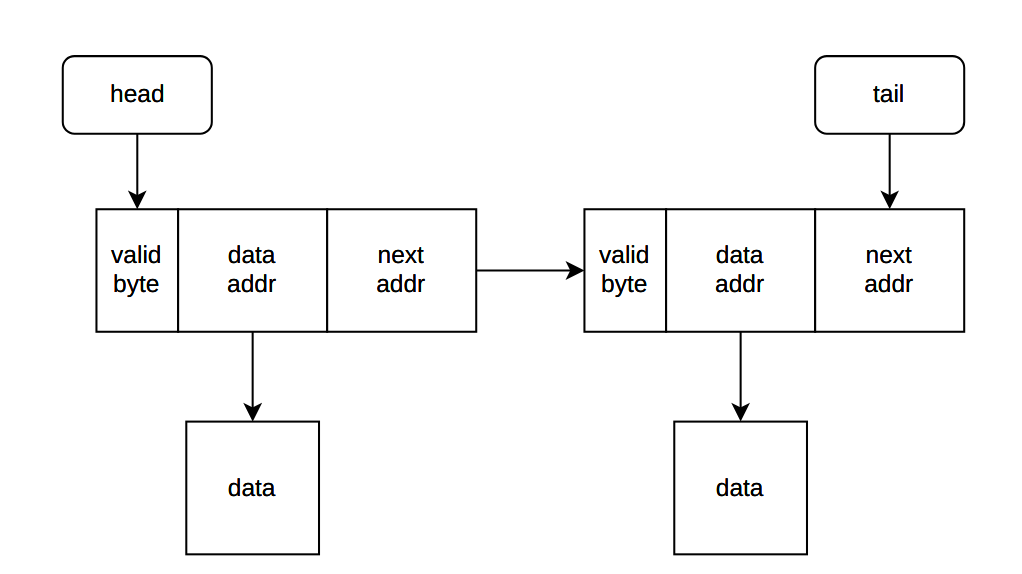
\includegraphics[width=8cm]{global_img_dir/linklist.png}
\end{frame}

\begin{frame}
    \frametitle{Buffer Pool: Valid Byte}
    \begin{block} {valid byte}
        \begin{itemize}
            \item data bit: If the data bit is equal to 1, the data addr is valid. Otherwise invalid
            \item next bit: If the next bit is equal to 1, the next addr is valid. Otherwise invalid
            \item used bit: If the used bit is equal to 1, this inode is used by some tasks
        \end{itemize}
    \end{block}
\end{frame}

\begin{frame}
    \frametitle{Buffer Pool: Automata}
    \begin{block} {valid byte}
        | used bit | next bit | data bit |
    \end{block}
    \centering
    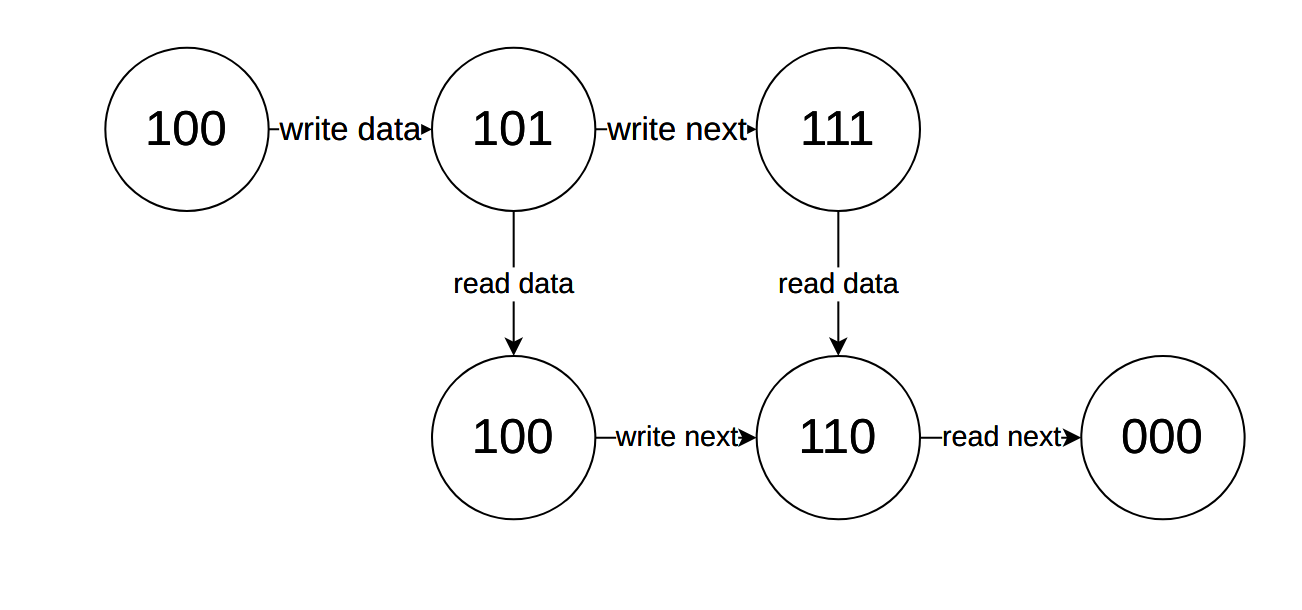
\includegraphics[width=12cm]{global_img_dir/automata.png}
\end{frame}


\begin{frame}[fragile]
    \frametitle{Buffer Pool: allocate inode}
    
        \begin{block} {case1}
            There is enough free space to allocate
        \end{block}
        \begin{lstlisting}[language=python]
    if inode_tail + inode_size > data_head:
        return inode_tail
        \end{lstlisting}

        \begin{block} {case2}
            Free Some unused inode
        \end{block}
        \begin{lstlisting}[language=python]
    for head in all_heads:
        if check_free(head) is True:
            return head
        \end{lstlisting}
        
\end{frame}

\begin{frame}[fragile]
    \frametitle{Buffer Pool: allocate data node}
    \begin{block} {case1}
        There is enough free space to allocate
    \end{block}
    \begin{lstlisting}[language=python]
if inode_tail + inode_size > data_head:
    return inode_tail
    \end{lstlisting}

    \begin{block} {case2}
        Free Some unused datanode
    \end{block}
    \begin{lstlisting}[language=python]
free = True
for datanode in all_datanodes:
    for ref in refs of datanode:
        if databit(ref) == 0 && dataaddr(ref) == datanode:
            free = False
            break
    if free is True:
        return datanode
    \end{lstlisting}
\end{frame}

\section{Experiment}
\begin{frame}
    \frametitle{Experiment}
    \begin{figure}[htbp]
        \centering
        \begin{minipage}[t]{0.48\textwidth}
        \centering
        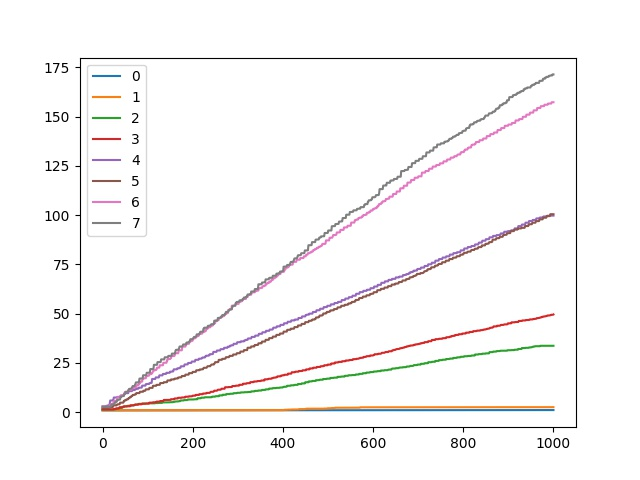
\includegraphics[width=6cm]{global_img_dir/l.jpg}
        \caption{time}
        \end{minipage}
        \begin{minipage}[t]{0.48\textwidth}
        \centering
        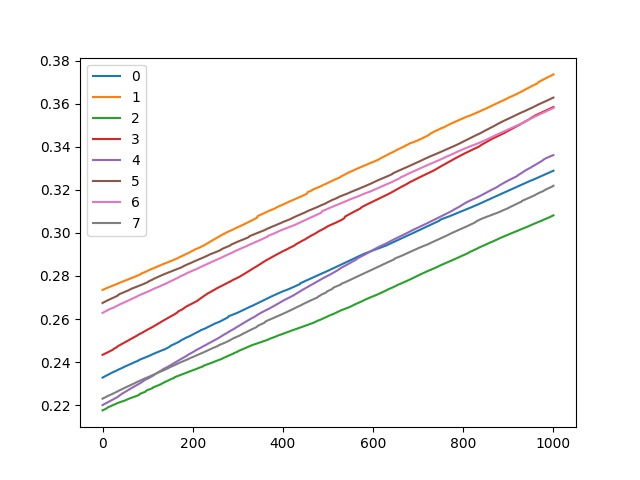
\includegraphics[width=6cm]{global_img_dir/gl.jpg}
        \caption{time with GlobalDataLoader}
        \end{minipage}
    \end{figure}
\end{frame}

\end{document}
